

\documentclass[sts]{article}
\usepackage[spanish]{babel}
\usepackage[hmargin=2.0cm,vmargin=1cm]{geometry}
\usepackage{graphicx}

\begin{document}

Punto 2 Taller 3 David Bernal Herramientas Computacionales

En la fig. \ref{fig:moon} se muestra la \textit{Estaci\'on Espacial Internacional} atravesando la Luna.

\begin{figure}[h]
\centering
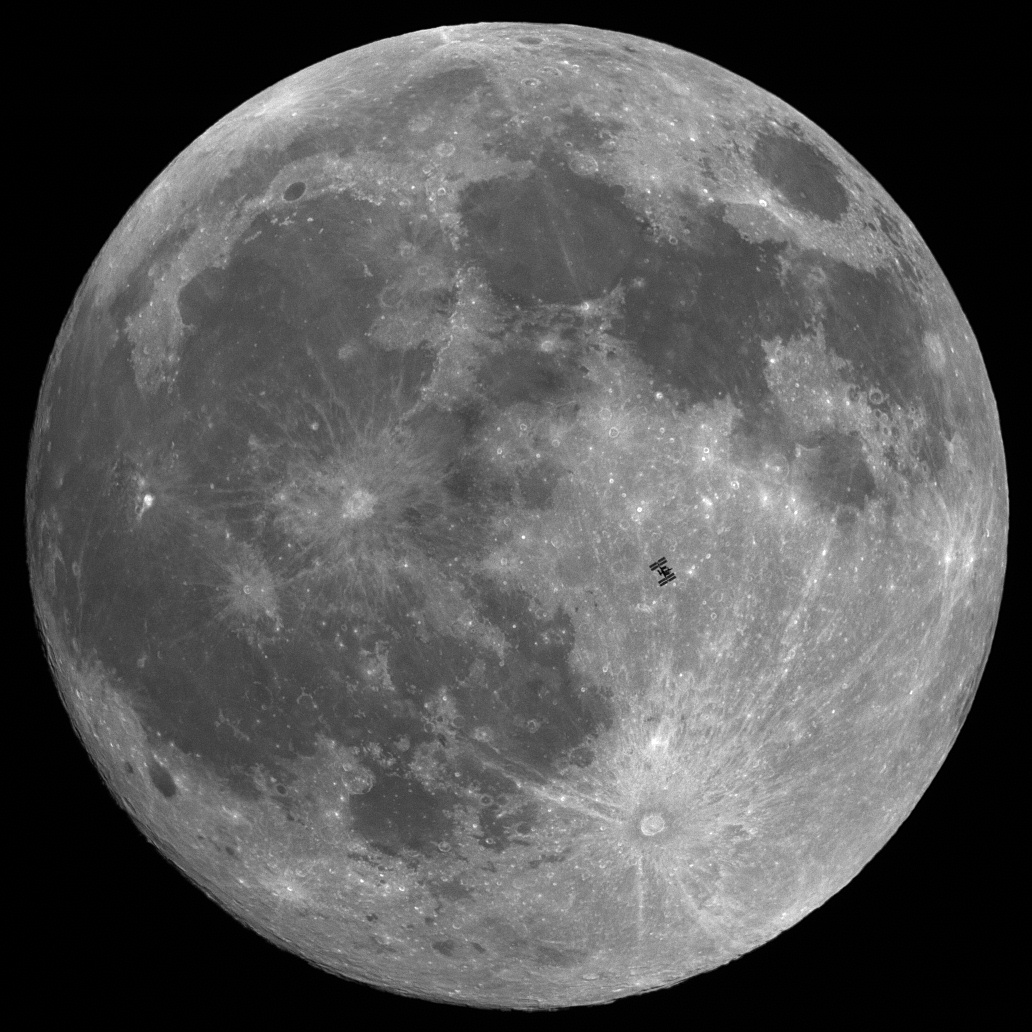
\includegraphics[scale=0.2]{ISS_moon.jpg}
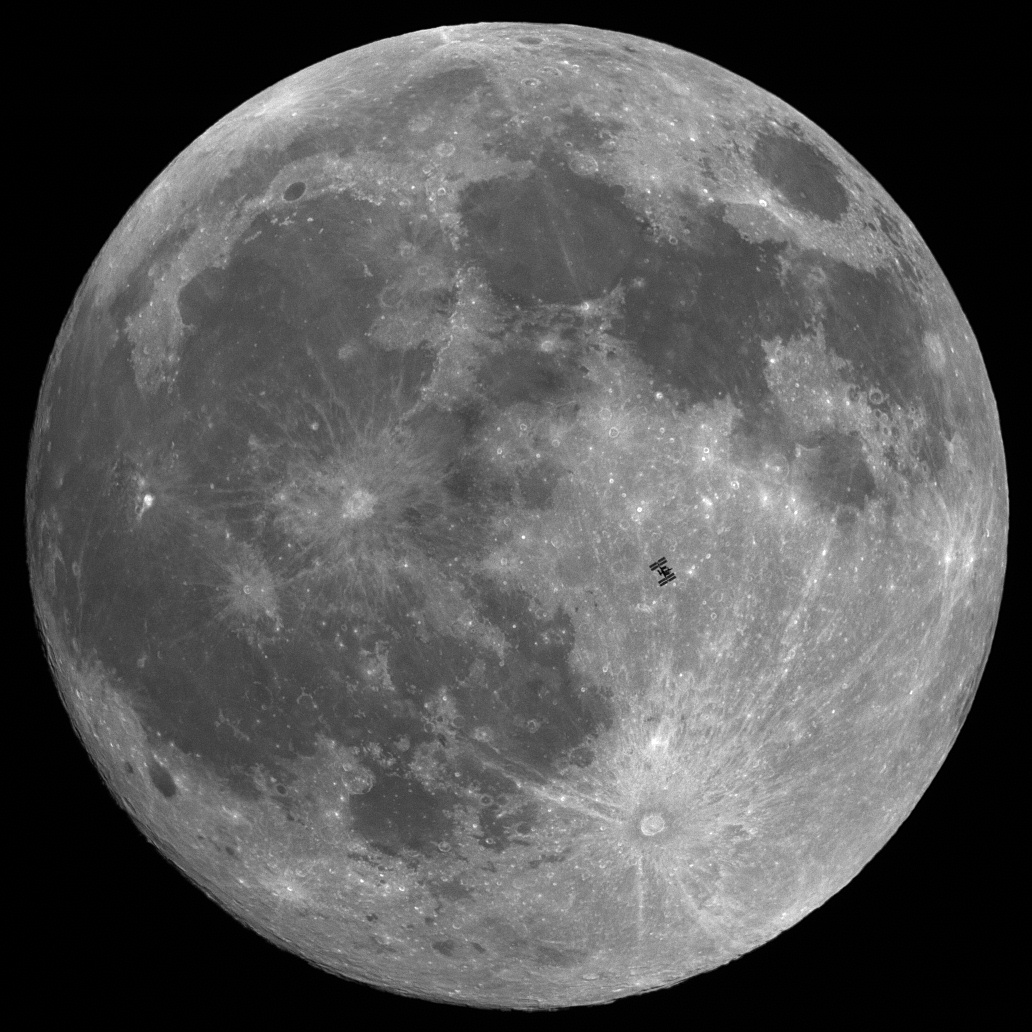
\includegraphics[scale=0.1]{ISS_moon.jpg}
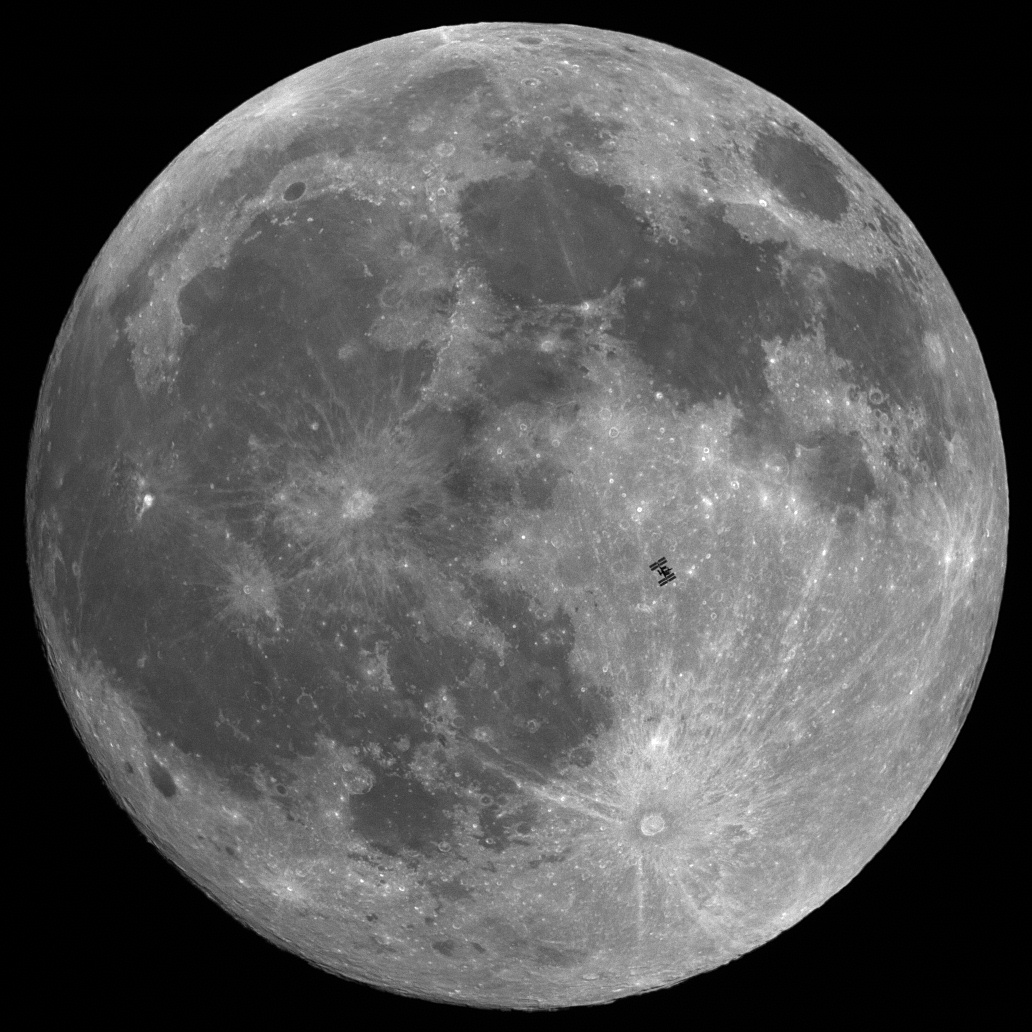
\includegraphics[scale=0.1,angle=45]{ISS_moon.jpg}
\caption{International Space Station (ISS), Moon transit.}
\label{fig:moon}
\end{figure}


\end{document}
